\documentclass[letterpaper]{article}

\usepackage{float}

\usepackage[margin=1in]{geometry} % full-width


% Unicodez, pdf metadata
\usepackage[utf8]{inputenc}
\usepackage{hyperref}
\hypersetup{
	unicode,
%	colorlinks, 
%	breaklinks, 
%	urlcolor=cyan, 
%	linkcolor=blue, 
	pdfauthor={Giovanna G. Amorim, Jonathan Loud, Jacob Rodriguez, Samuel-José Turcotte},
	pdftitle={BIO CE Project - [Title]},
	pdfsubject={},
	pdfkeywords={},
	pdfproducer={Giovanna G. Amorim, Jonathan Loud, Jacob Rodriguez, Samuel Turcotte},
	pdfcreator={Giovanna G. Amorim, Jonathan Loud, Jacob Rodriguez, Samuel Turcotte}
}

%graphics
\usepackage{graphicx}
\graphicspath{ {./figs/} }

%references
\usepackage{biblatex} %Imports biblatex package
\addbibresource{Bio-ce.bib}

%math stuff
\usepackage{algorithm, algpseudocode} % use algorithm and algorithmicx for typesetting algorithms
\usepackage{mathrsfs} % for \mathscr command
\usepackage{amsmath}


%graph stuff
\usepackage{pgfplots}
\pgfplotsset{width=15cm,compat=1.9}

\usepgfplotslibrary{external}
\tikzexternalize

\usepackage{booktabs}


% cover page
\title{On the Laboratory Synthesis of Electric Eel Electrocytes}
\author{Jonathan Loud 2342270, Jacob Rodriguez 2336804, \\
Giovanna G. Amorim 233 4984, Samuel-José Turcotte 2339779}

\date{Dawson College \\[25pt]
000-000-000 section 00001\\[25pt]
Dr. Jeffery K. Eng\\[25pt]
Submission: \today}

\begin{document}

\maketitle

\begin{abstract}
    This paper explores the experimental simulation of electric eel cells. By simulating the electrochemical 
	conditions found within eel electrocytes on a macroscopic scale, this experiment was able to produce 
	significant voltages ranging in the hundreds of millivolts. Specifically, this experiment employed 
	the use of sodium alginate, an organic salt that releases Na+ ions in water, to simulate the release of sodium 
	ions in electrocytes. By using dialysis tubing with a specific pore size, it was possible to trap the alginate 
	while allowing the diffusion of Na+, thereby creating a charge differential across the tubing and inducing a measurable
	voltage.
	\noindent\textbf{Keywords:} Battery, Dialysis Membrane, Dialysis Tubing, Eel, Electric Eel, Electrocyte, Sodium Alginate, Voltage
\end{abstract}

\tableofcontents

\newpage

\section{Introduction}
\label{sec:introduction}

Native to the freshwater rivers of South America, the \textit{Electrophorus electricus}, or more 
commonly referred to as the electric eel, is known for its ability to generate high voltage shocks,
formally known as electric organ discharges (EOD); these EODs can be classified into low-voltage 
EODs and high-voltage EODs. Low-voltage EODs are expressed at lower frequencies of about 10Hz to
20Hz \parencite{cataniaAstonishingBehaviorElectric2019}, reaching about 10 V \parencite{ElectricCircuits6ElectricEels2015}. 
Therefore, they are more practical for communication and determining the presence of organisms 
in their environment through a process called electrolocation: monitoring 
changes in a particular electric field \parencite{bennettComparativePhysiologyElectric1970}. 
On the other hand, high-voltage EODs are used as an attack or defence mechanism,
the largest recorded voltage discharge being 500V \parencite{ElectricCircuits6ElectricEels2015}.
However, whether the emitted EODs are expressed as low or high 
voltages, they are produced from a specific cell that makes up 80\% of the eel’s body: electrocytes
\parencite{carlsonAnimalBehaviorElectric2015}. These electrocyte cells are arranged in series and 
in parallel and are located in the electric eel’s three most prominent organs: Sach’s organ, the 
Main organ, and Hunter’s organ \parencite{ElectricCircuits6ElectricEels2015}. [cite this figure (Figure 1.)] This 
arrangement allows for the entire eel to be viewed as a battery, with the positive and negative 
poles at the head and tail respectively, allowing for the variety of EOD voltages mentioned above. 
Although electric eels have the potential to release high-voltage EODs, the current produced remains
nonetheless quite minimal (~1 A) \parencite{ElectricCircuits6ElectricEels2015}. This is a result 
of the high resistance of the freshwater where these eels are found, or more precisely, the lack of 
ions to maintain the electric current \parencite{boisseletBiomimeticPotentialElectric2017}. 
Consequently, to optimize the battery potential of the electric eels EOD, research was conducted 
by Lina Guezi \parencite{gueziTheoreticalExaminationConception2023}, a collegue of ours, to produce 
a synthetic replication of the electric eel’s electrocyte 
cells in ionized water. Our experiment aims to test their research findings by making our own battery prototype based off of their work with a few modifications in order to explore 
the potential uses of this biological battery. To do so we used a dialysis membrane to isolate positive sodium ions ( $Na^+$), similarly to how the electric eels do in their
electrocyte cells, which creates a potential gradient across our synthetic electrocyte cell.
This process generates a voltage difference which then produces an electric discharge, 
similarly to a battery. The synthetic batteries created in this lab function through the
principles of diffusion and dissociation. 

\begin{figure}[H]
	\centering
	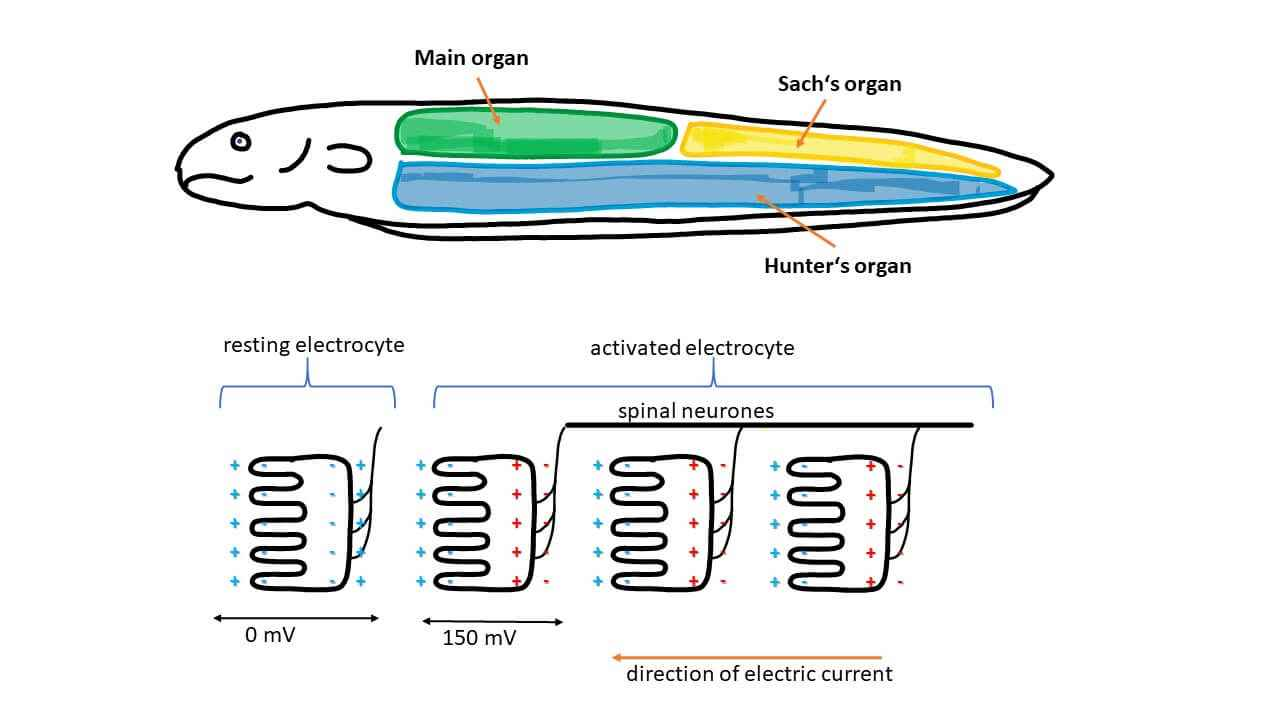
\includegraphics[width=0.60\textwidth]{fig1.jpg}
	\caption{Electric eel's organ composition (Hunter's organ, the Main organ, and Sach's organ make up 80\% of the eel's organs) with electrocyte cell alignment and polarization.}
	\label{fig:1}
\end{figure}

Firstly, the salt used in this experiment is sodium 
alginate. Like all salts, sodium alginate is composed of a positively-charged cation (in this case, sodium),
and a negatively-charged anion (here, alginic acid). These two components are fused together in solid 
form by an ionic bond. However, when placed in an aqueous environment, the ionic bond is broken and 
the two components are allowed to separate. This phenomenon occurs in most salts, and is known as 
dissociation. Next, this experiment uses diffusion and a semi-permeable membrane to separate the charged 
ions. The sodium alginate is held in a capsule made of dialysis tubing, a specialized membrane with 
microscopic pores. These pores are of a very particular size, as to allow certain smaller molecules to 
pass freely across the membrane, while blocking larger molecules from crossing. This is known as a 
semi-permeable membrane. The membrane used in this experiment has a molecular cut-off weight between 
6,000 and 8,000 Daltons. This means that 90\% of molecules with a molecular weight greater than 8,000 
Daltons will be trapped by the membrane \parencite{MolecularWeightCut2014}. In the case of alginic acid, 
which possesses a molecular weight between 10,000 and 600,000 Daltons 
\parencite{MolecularWeightDetermination}, the membrane is non-permeable. This means that the alginic 
acid ions placed within the tubing will remain. However, the sodium ions released are quite small, with 
a mass of around 23 Daltons. Therefore, they are free to diffuse across the membrane into the surrounding 
water. Taking into account the fact that sodium ions possess a charge of 1+, and the alginic acid, 
therefore, possesses a charge of 1-, as sodium ions begin to diffuse across the membrane, the water 
outside the tubing acquires a positive charge. Likewise, the solution within the tubing starts to 
contain more alginic acid than sodium and therefore goes from a neutral solution to becoming 
negatively charged. This charge imbalance is then measurable by using a voltmeter.


\section{Material and Methods}
\label{sec:matandmet}

\subsection*{Materials}

\begin{itemize}
	\item Drinking glasses or other receptacles capable of holding water
	\item Dialysis tubing with a MWCO of 6-8kDa
	\item Sodium alginate powder
	\item Voltmeter
	\item Alligator wires
\end{itemize}

\subsection*{Method}

\begin{enumerate}
	\item Drinking glasses were rinsed and filled with hot tap water. Roughly 10cm pieces of dialysis tubing were cut, and one piece of tubing was soaked in each glass for 30 minutes.
	\item Dialysis tubing pieces were removed from the water, opened up, and a knot was tied at the bottom of each piece, sealing it. 1.25mL of sodium alginate powder was inserted into each section of tubing, and the tubes were filled around 3/4 of the way with water to dissolve the powder. Stirring rods were used to aid soaking and dissolution of the powder.
	\item The filled dialysis membranes were placed back into their glasses, open side up, ensuring that the top of each piece protruded past the water level in the glasses.
	\item The setup was left for 12 hours to maximize ionic diffusion.
	\item The voltage of each sample was measured by placing two alligator-clip wires in each glass: one wire was placed inside the dialysis tubing, and one was placed in the glass but outside the tubing. The positive probe of the voltmeter was then attached to the wire outside the tubing, and the negative probe was connected to the wire inside the tubing. A reading was then made using the voltmeter and the data was recorded. This was repeated for each replicate.
\end{enumerate}

%figures

\begin{figure}
	\centering
	\includegraphics[width=0.60\textwidth]{fig2.png}
	\caption{Experiment with aluminium foil attached to electrode}
	\label{fig:2}
\end{figure}

\begin{figure}
	\centering
	\includegraphics[width=0.40\textwidth]{fig3.png}
	\caption{Membranes being left to diffuse}
	\label{fig:3}
\end{figure}


\section{Results and Discussion}
\label{sec:results and Discussion}


\begin{table}[]
	\begin{tabular}{ccc}
	\hline
	Quantity of Sodium Alginate (mL) & Initial voltage (mV) & Voltage after 12 hours (mV) \ \hline
	0                                & 1.2                  & 2.6                         \
	0                                & 1.8                  & 3.7                         \ \hline
	1.25                             & 38                   & 101                         \
	1.25                             & N/A                  & 39                          \
	1.25                             & N/A                  & 46                          \ \hline
	2.5                              & 40.9                 & 26.4                        \
	1.25 (with aluminium)            & 639                  & 141                         \ \hline
	\end{tabular}
	\caption{Voltage measured according to the quantity of sodium alginate added}
	\label{tab:my-table}
\end{table}


\begin{table}[]
	\begin{tabular}{ccc}
	\hline
	Quantity of Sodium Alginate (mL) & Initial voltage (mV) & Voltage after 12 hours (mV) \ \hline
	0                                & 1.2                  & 2.6                         \
	0                                & 1.8                  & 3.7                         \ \hline
	1.25                             & 38                   & 101                         \
	1.25                             & N/A                  & 39                          \
	1.25                             & N/A                  & 46                          \ \hline
	2.5                              & 40.9                 & 26.4                        \
	1.25 (with aluminium)            & 639                  & 141                         \ \hline
	\end{tabular}
	\caption{Voltage measured according to the quantity of sodium alginate added}
	\label{tab:my-table}
\end{table}

The results obtained by the lab indicate that the voltages produced by the experimental replicates (M=81.82mV, SD=20) are significantly greater than those generated by the control group t(4) = -2.6, p = .048. This confirms the hypothesis that if sodium alginate is dissociated inside a dialysis membrane, by diffusion, a potential difference will be created across the membrane.

Our experiment created a voltage using a reaction similar to an electrolyte in an electric eel. By releasing sodium alginate, an ionic molecule that dissociates into two oppositely charged particles of different sizes, we were able to separate the sodium cations from the algin anions, thus creating a difference in charge inside and outside the membrane. This created a difference of potential and voltage. The initial voltage measured was significantly higher than the control (38mV, 639mV, and 40.9mV). After 12 hours, the voltage was also higher than the control (101.26,141,39mV, 46mV, and 26.4 mV). This yields a p-value of .048, less than the general α value of 0.05, and therefore the results are said to be statistically significant. Additionally, our data suggests that the voltage after 12 hours is lower than that measured immediately after the dissolution of the sodium alginate. This voltage drop may be due to the dialysis membrane pore size. If the pores are too large, it may be possible for small quantities of alginic acid to slowly diffuse across the membrane. We also observed that adding aluminum foil to the end of the electrode of the voltmeter seems to significantly increase the voltage. Unfortunately, as we were limited by the quantity of materials, we did not perform multiple replicates of this. Having 2.5mL of sodium alginate also does not seem to significantly affect the voltage measured, though this result is not yet conclusive.

We noticed that the current is very low and decreases rapidly. When measured, the voltage would drop significantly during the time it was being measured. This is similar to the voltage produced by electric eels which can produce high voltages but for a very short time. Even at its most stable, the voltage fluctuated greatly. Therefore, the noted results have an uncertainty of \pm 10mV due to this fluctuation.

To further explore the potential of these batteries, it would be useful to make more replicates. Due to the limited quantity of membrane, we were limited to seven attempts. By experimenting with different procedures, we refined our protocol to give the best results. If we were to redo this experiment, we would only use 1.25 mL of sodium alginate, as 2.5 mL overflows easily and is quite viscous, making mixing the solution challenging. Placing aluminum foil on the electrodes could be another solution, as it would increase the surface area to which ions can attach allowing for a higher generated voltage. Additionally, it may be possible to measure the voltage more frequently to find the time at which the charge differential across the membrane was the greatest. If we were to make a graph showing the progression of voltage over time, it may be possible to maximize the voltage. It may also be interesting to put multiple cells in series to generate an even higher voltage.


\printbibliography[heading=bibintoc]

\end{document}

